
\section{Performance of \shortname\ with varying sentence lengths}
    In this experiment, we measure the performance of baseline and our models by testing on sentences of varying lengths. We partition the original CaRB test data into 6 datasets with sentences of lengths (9-16 words), (17-24 words), (25-32 words), (33-40 words), (41-48 words) and (49-62 words) respectively. Note that the minimum and maximum sentence lengths are 9 and 62 respectively. We measure the Optimal F1 score of both Copy Attention + BERT and IMOJIE (Bootstrapped on OpenIE-4) on these partitions as depicted in Figure \ref{fig1}. \newline

    We observe that the performance deteriorates with increasing sentence length which is expected as well. Also, for each of the partitions, IMOJIE marginally performs better as compared to Copy Attention + BERT.

    \begin{figure}[h]
    \begin{center}
    \advance\leftskip-3cm
    \advance\rightskip-3cm
    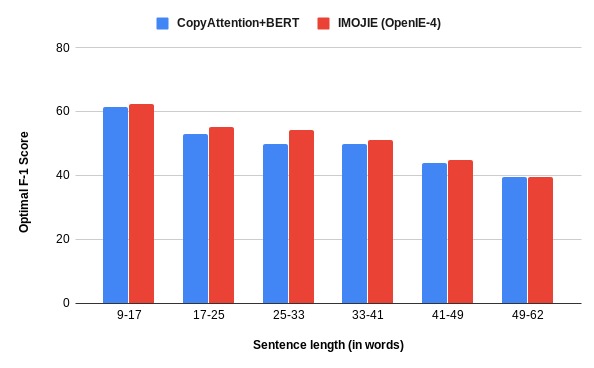
\includegraphics[keepaspectratio=true,scale=0.35]{images/imojie/Fig1.png}
    \caption{Measuring performance with varying input sentence lengths}
    \label{fig1}
    \end{center}
    \end{figure}
    
\section{Measuring Performance of \shortname\ on Varying Beam Size}
    We perform inference of the CopyAttention with BERT model on CaRB test set with beam sizes of 1, 3, 5, 7, and 11. We observe in Figure \ref{fig2} that AUC increases with increasing beam size. A system can surge its AUC by adding several low confidence tuples to its predicted set of tuples. This adds low precision - high recall points to the Precision-Recall curve of the system leading to higher AUC.\\
    On the other hand, Last F1 experiences a drop at very high beam sizes, thereby capturing the decline in performance. Optimal F1 saturates at high beam sizes since its calculation ignores the extractions below the optimal confidence threshold.\\
    This analysis also shows the importance of using Last F1 as a metric for measuring the performance of OpenIE systems.
    
    \begin{figure}
    \begin{center}
    \advance\leftskip-3cm
    \advance\rightskip-3cm
    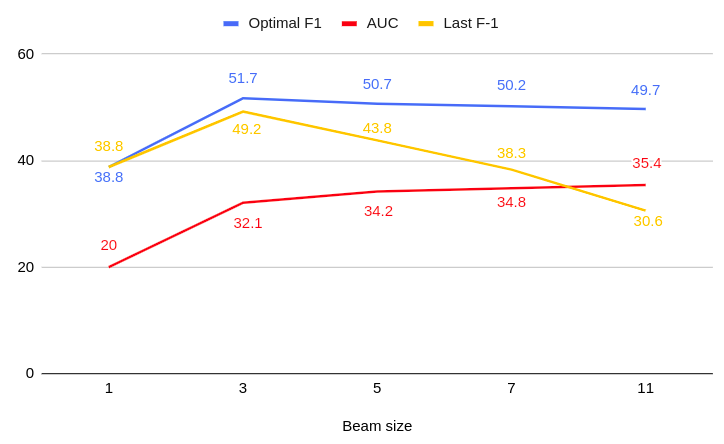
\includegraphics[keepaspectratio=true,width=\hsize]{images/imojie/Fig2.png}
    \caption{Measuring performance of CopyAttention with BERT model upon changing the beam size}
    \label{fig2}
    \end{center}
    \end{figure}
    
    \begin{table*}
    \begin{center} {\footnotesize
    \begin{tabular}{lccc}
    \hline
     \textbf{Model} & \multicolumn{3}{c}{\textbf{Dataset}}  \\
     & \multicolumn{1}{c}{Wire57} & \multicolumn{1}{c}{Penn} & \multicolumn{1}{c}{Web}\\
    \hline 
    CopyAttention + BERT & 45.60, \textbf{27.70}, 39.70 & 18.20, 7.9, 12.40 & 30.10, \textbf{18.00}, 14.60 \\ 
    \shortname & \textbf{46.20}, 26.60, \textbf{46.20} & \textbf{20.20}, \textbf{8.70}, \textbf{15.50} & \textbf{30.40}, 15.50, \textbf{26.40} \\ \hline
    \end{tabular} }
    \end{center}
    \caption{Evaluation on other datasets with the CaRB evaluation strategy}
    \label{tab:ODE}
    \end{table*}
    
\section{Evaluation of \shortname\ on other datasets}
    
    We use sentences from other benchmarks with the CaRB evaluation policy and we find similar improvements, as shown in Table \ref{tab:ODE}. \shortname{} consistently outperforms our strongest baseline, CopyAttention with BERT, over different test sets. This confirms that \shortname{} is domain agnostic.
    
\section{Visualizing Attention}
    \label{sec:visualize_attention}
    
    Attention has been used in a wide variety of settings to help the model learn to focus on important things \cite{bahdanau&al15, xu&al15, lu&al19}. However, the \shortname{} model is able to use attention to understand which words have already been generated, to focus on remaining words. In order to understand how the model achieves this, we visualize the learnt attention weights. There are two attention weights of importance, the learnt attention inside the BERT encoder and the attention between the decoder and encoder.  We use BertViz \cite{vig@19} to visualize the attention inside BERT.
    
    We consider the following sentence as the running example - "he served as the first prime minister of australia and became a founding justice of the high court of australia". We visualize the attention after producing the first extraction - ``he; served; as the first prime minister of australia''. Intuitively, we understand that the model must focus on the words ``founding'' and ``justice'' in order to generate the next extraction - ``he; became; a founding justice of the high court of australia''. In Figure \ref{fig:prime} and Figure \ref{fig:minister} (where the left-hand column contains the words which are used to attend while right-hand column contains the words which are attended over), we see that the words ``prime'' and ``minister'' of the original sentence have high attention over the same words in the first extraction. But the attention for ``founding'' and ``justice'' are limited to the original sentence.
    
    Based on these patterns, the decoder is able to give a high attention to the words ``founding'' and ``justice'' (as shown in Figure \ref{fig:att_weights}), in-order to successfully generate the second extraction "he; became; a founding justice of the high court of australia".
    
    \begin{figure}
    \begin{center}
    \advance\leftskip-3cm
    \advance\rightskip-3cm
    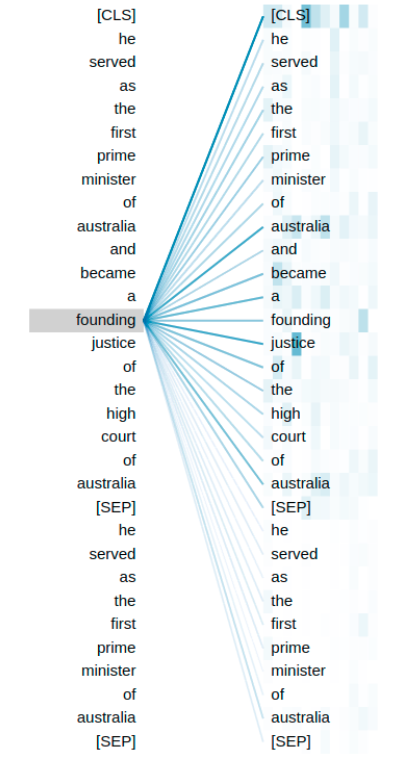
\includegraphics[keepaspectratio=true,width=0.5\vsize]{images/imojie/founding_cut.png}
    \caption{BERT attention for the word `founding'}
    \label{fig:founding}
    \end{center}
    \end{figure}
       
    \begin{figure}
    \begin{center}
    \advance\leftskip-3cm
    \advance\rightskip-3cm
    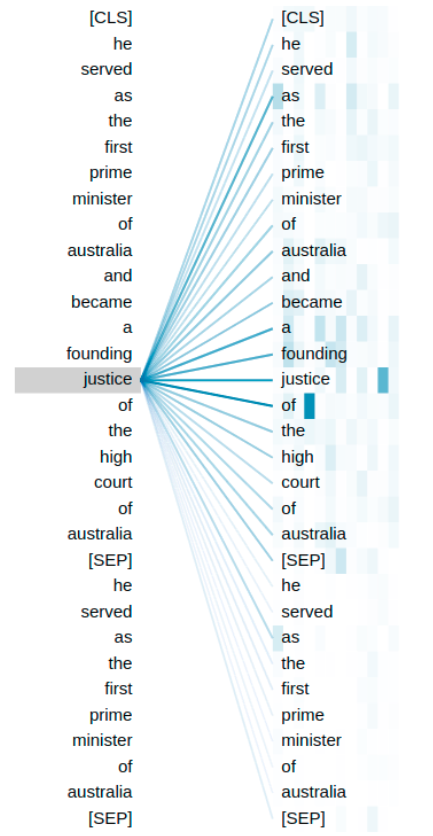
\includegraphics[keepaspectratio=true,width=0.5\hsize]{images/imojie/justice_cut.png}
    \caption{BERT attention for the word `justice'}
    \label{fig:justice}
    \end{center}
    \end{figure}
    
    \begin{figure}
    \begin{center}
    \advance\leftskip-3cm
    \advance\rightskip-3cm
    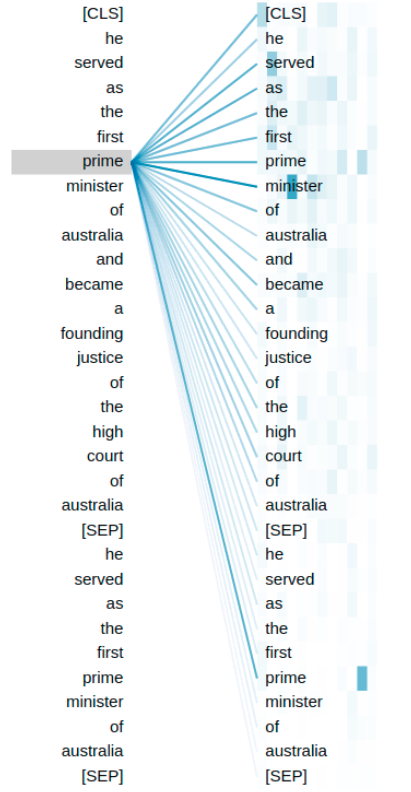
\includegraphics[keepaspectratio=true,width=0.5\hsize]{images/imojie/prime_cut.png}
    \caption{BERT attention for the word `prime'}
    \label{fig:prime}
    \end{center}
    \end{figure}
    
    \begin{figure}
    \begin{center}
    \advance\leftskip-3cm
    \advance\rightskip-3cm
    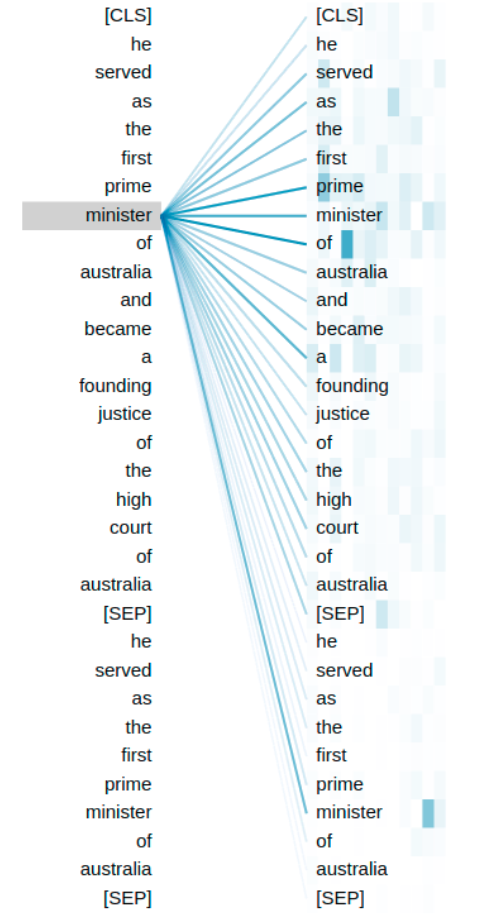
\includegraphics[keepaspectratio=true,width=0.5\hsize]{images/imojie/minister_cut.png}
    \caption{BERT attention for the word `minister'}
    \label{fig:minister}
    \end{center}
    \end{figure}
    
    \begin{figure*}
    \begin{center}
    \advance\leftskip-3cm
    \advance\rightskip-3cm
    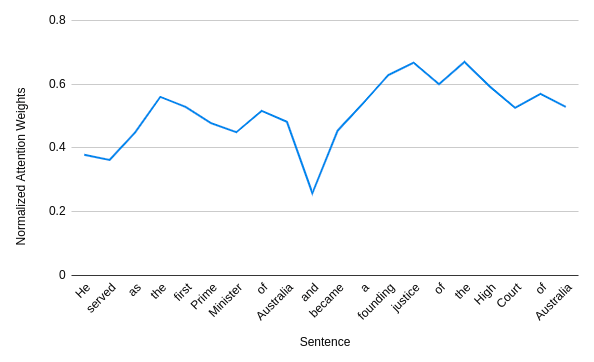
\includegraphics[keepaspectratio=true,width=\hsize]{images/imojie/att_weights.png}
    \caption{Attention weights for the decoder}
    \label{fig:att_weights}
    \end{center}
    \end{figure*}